\documentclass[onecolumn]{elsarticle}

\usepackage{amssymb}
\usepackage{graphicx}
\usepackage{caption}
\usepackage{subcaption}
\usepackage{rotating}
%\usepackage[font=small,labelfont=bf,tableposition=top]{caption}
\usepackage{booktabs}
\usepackage{lineno}
%\biboptions{longnamesfirst,angle,semicolon}

\journal{Renewable \& Sustainable Energy Reviews}


%\usepackage{algorithm}
%\usepackage{algorithmic}
\usepackage[lined, ruled, linesnumbered]{algorithm2e}

%\usepackage{hyperref}
\usepackage[pdftex]{hyperref}
% \hypersetup{colorlinks, sitecolor=black, pdftex}
\hypersetup{colorlinks,%
citecolor=black,%
filecolor=black,%
linkcolor=black,%
urlcolor=black}%,%
% pdftex}


%\usepackage{ecj,palatino,epsfig,latexsym,natbib}
\usepackage[latin1]{inputenc}
%\usepackage[utf8]{inputenc}
\usepackage{algorithmic}
%\usepackage[algoruled,lined, boxed]{algorithm2e}
%\usepackage{indentfirst} %Indentar primeiro paragrafo
\usepackage{amsmath}
\usepackage{amssymb}


\usepackage{rotating}
\usepackage{natbib}

\begin{document}

\begin{frontmatter}

\title{Survey and trends on Multi-Agent Systems applications in Smart-Microgrids}


\author[ufmgGrad,ipdt]{Vitor N.~Coelho\corref{cor1}}
\ead{vncoelho@ufmg.br,vncoelho@gmail.com}

\author[ufmg]{Frederico G.~Guimar�es}

\author[braude]{Miri Weiss Cohen}
%\ead{marcone@iceb.ufop.br}

\author[ufopDECAT]{Agnaldo J. R. Reis}
%\ead{agnreis@gmail.com}

\author[ufmg]{Sidelmo M. Silva}
%\ead{agnreis@gmail.com}

% \author[ufopDECOM]{Marcone J.F.~Souza}
% \ead{marcone@iceb.ufop.br}

\cortext[cor1]{Corresponding author. Address: Department of Electrical Engineering, Federal University of Minas Gerais, Belo Horizonte, MG, 31270-010,
Brazil. Tel + 55 31 35514407. Fax + 55 31 35514407.}


\address[ufmgGrad]{Graduate Program in Electrical Engineering, Universidade Federal de Minas Gerais, Belo Horizonte, Brazil}
\address[ufmg]{Department of Electrical Engineering, Universidade Federal de Minas Gerais, Belo Horizonte, Brazil}
\address[braude]{Department of Software Engineering,  ORT Braude College of Engineering, Karmiel, Israel}
\address[ufopDECAT]{Department of Control and Automation Engineering,  Universidade Federal de Ouro Preto, Ouro Preto, Brazil}
%\address[ufopDECOM]{Department of Computer Science,  Universidade Federal de Ouro Preto, Ouro Preto, Brazil}





\begin{abstract}
Smart-microgrid is a potential solutions being studied for future distributed generation systems.
Due to the distributed topology of the emerging Smart Grid (SG) systems, the paradigm of Multi-Agent Systems (MAS) has been showing an useful tool that has been addressed in different applications. 
In this paper, the major issues and challenges in MAS and smart-microgrids are discussed, 
and a review of state-of-the-art applications and trends is presented.
\end{abstract}

\begin{keyword}
Smart Grid \sep
Microgrid \sep
Multi-Agent Systems \sep
Smart-microgrids 
\end{keyword}


\end{frontmatter}

\tableofcontents


%%%%%%%%%%%%%%%%%%%%%%%%%%%%%%%%%%%%%%%%%%%%%%%%%%%%%%%%%%%%%%%%%%%%

\section{Introduction}
\linenumbers

Smart grid is considered as a future of power grid which is able to manage the production, transmission and distribution of electricity by 
using information technology, distributed systems and artificial intelligence.
SG has become a major challenge for developed and developing nations in both research and utilization aspects \cite{Fadaeenejad2014,Tugcu2012}.
It is expected to play an important role order to resolve many issues of current power grid systems \cite{Fadaeenejad2014}.
The latter will be now composed of a mesh of networked MG collaborating to deliver electricity to consumers \cite{Merabet2014Applications}. 

%specially, in developing countries \cite{Pereira2012,Diaz2013,Pao2013,PereiraJr2013,AlemanNava2014Mexico,Yuan2014,Lin2013,Welsch2013,Acharjee2013}
Future MG may equip customers with distributed generation and storage systems that can change their overall demand behavior.
Rogers, Ramchurn \& Jennings \cite{Rogers2012-Challenges} highlighted that demand side, the consumers,
will have to adapt to the available resources, in contrast to the current model in which the supply should always match the demand.
Providing autonomous assistance in order to assist complex decision making tasks will be required by an increasing number of MG users.

The need of reducing environmental impacts, as emissions of greenhouse gases, motivate the growth of Renewable Energy Resources (RER) based systems \cite{PereiraJr2013,Welsch2013, Lin2013}.
The potential for RER is growing quick and it is expected that it will exponentially exceed the world's energy demand \cite{Ellabban2014}.
SG's infrastructure should also provides new opportunities for the grid and its customers for information exchange regarding real-time electricity rates and demand profiles. \cite{Kahrobaee2014}.
Energy management system of SG is tightly associated with the communications between stakeholders and entities. 
Providing essential infrastructure for consumers and stakeholders to monitor and control their energy production and usage should be taken into account over the new systems.

%Due to the distributed topology of the emerging smart grids system, 
%the paradigm of Multi-Agent Systems (MAS) has been showing an useful tool that has been addressed in different applications. 

% The Smart Grids (SGs) are regarded as the new
% SG. MAS constitute a new field of research in full effervescence
% generation of electric power systems, combining the development and technological development. MAS are particularly useful for
% of Information Technology (IT), distributed systems and Artificial designing distributed systems requiring autonomy of their
% Intelligence (AI) for more features on the real-time monitoring of entities (e.g., bargaining agents, drones, etc.). MAS use new
% the Demand / Response (DR) and the energy consumption
% 

Coordination and controlling of all these new emerging components remains a great challenge.
Advanced networking, as well as information and communication technologies (ICTs), have been motivating 
the integration of the conventional power grid in smarter ways \cite{Nguyen2012AgentBasedRestorationSG}, known as a peer-to-peer or distributed multi-agent system (MAS).
Autonomous control of SG system allows placing additional DGs without reengineering the system, and using it in the peer-to-peer model eliminates the requirement of a complex central
controller and associated telecommunication facilities \cite{Lidula2011TestSystemMG}.
MAS is one of the most fastest growing domains in agent oriented technology which deals with modeling of autonomous decision making entities \cite{Logenthiran2008},
which have been showing to be crucial in SG operations.

The need to integrate both field of knowledge, MAS and SG, have increased extensively in recent years around the world.
Figure \ref{fig:searchMASSG} shows the number of publications relating MAS and SG in the Scopus database, performed in 9th, April, 2015.

 \begin{figure}[htbp]
\centering	
	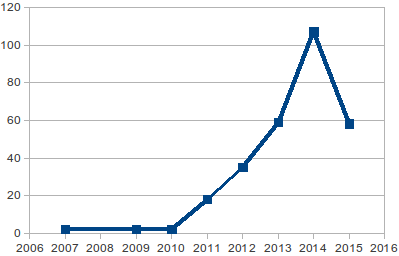
\includegraphics[scale=0.5]{./figs/searchSCOPUS-MAS-SG.png}
	\caption{ \label{fig:searchMASSG}}	
\end{figure}

In particular, the MAS paradigm can be adapted to model, control, manage or test the operations and management of MG . 
MG had become a basic and fundamental infrastructure in the SG environment and have been receiving attention in recent literature works \cite{Coelho2014WCCI,Chen2013}.
Microgrid is been intensively studied as a possible future energy system paradigm and its control.
As noticed by Jiayi, Chuanwen \& Rong \cite{Jiayi2008}, MAS technology can be applied in it in order to solve number of specific operational problems, such as:
``First of all, small Distributed Energy Resources (DER) units have different owners, and several decisions should be taken locally
so centralized control is difficult. Furthermore MGs operate in a liberalized market;
therefore the decisions of the controller of each unit concerning the market should have a
certain degree of ''intelligence``. Finally the local DER units besides selling power to the
network have also other task: producing heat for local installations, keeping the voltage
locally at a certain level or providing a backup system for local critical loads in case of a
failure of the main system''
MG systems aggregates many DER and loads together as an autonomous entity \cite{Zheng2010}.
Its use in microgrid has been tackled by different researches and still a complex task \cite{Logenthiran2008}.
Figure \ref{fig:searchMASMG} shows the number of publications relating MAS and MG.

 \begin{figure}[htbp]
\centering	
	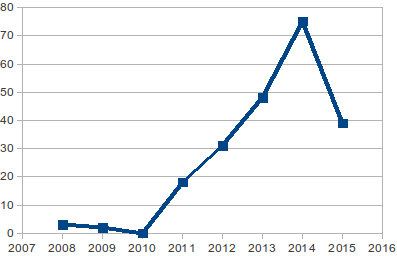
\includegraphics[scale=0.5]{./figs/searchSCOPUS-MAS-MG.png}
	\caption{ \label{fig:searchMASMG}}	
\end{figure}


The interesting in developing applications involving MAS paradigm is also founded by private sectors,
where some patents have been registered in the last years.
A patent consisted in a method configured for execution in a computing device in a microgrid, the computing device assigned to a particular power source in the microgrid
was registered by \cite{goldsmith2012computingPatent}.
Another one, by...


%The use of storage allows both sides, demand and production, to optimize the power exchanged with
%the main grid, in compliance with the electricity market and forecasts.
%Renewable energy generators associated with storage units are considered as active distributed generators, one of
%the fundamental elements of power management in MG systems.

%In this regard, storage is able to increase renewable energy self-consumption and independence from the grid.










% 
% ``The SG components are often distributed and the energy 
% management system is tightly associated with the 
% communications between stakeholders and entities
% (agents) to exchange information. 
% MAS are by nature
% distributed and concurrent, they are independent entities
% engaged in the system, they have their own perception
% of the environment, goal and agenda and they try to
% achieve the best for themselves while behaving strategically. 
% Therefore, in that case when using MAS the amount of data to be disseminated (with its according costs) will be greatly reduced in comparison
% to other in-depth communication methods.''
% 
% SG is a holistic system and the failure of some part of it
% (the breakdown of a transmission line or cut down of a
% substation, transformer. . . .) shouldn't affect the whole
% activities and operations. Flexibility denotes the ability
% of a system to be adaptable (i.e., to behave as required
% in different situations). The flexibility of MAS is given
% by the fact that agents are independent and able to
% perceive their environment and then adapt their actions
% accordingly.
% 
% ``SG should demonstrate the plug-and-play concept for 
% integrating energy storage, loads, and sources at the 
% building level with the external utility grid. Plug and 
% play adaptability is widely proven by MAS, by nature 
% MAS are able to be scaled up by adding other agents or 
% by dispersing them in new environment with new 
% resources and capacities. ''
% 
% As SG will be composed for an aggregate of Microgrid,
% the control can be delegated to micro grids. In this
% vision, the MAS can perform tasks locally if they have
% sufficient knowledge and resources, and they can
% interact with other surrounding agents to help in the
% completion of tasks or decisions. The problem of control
% can be approached from a variety of perspectives
% including cognitive science, heuristic search and
%  machine learning.
%  
%  
%  SG leverage the widespread of the information and
% communication technologies, these smart technologies
% are platform-independent and language free. In this
% perspective, an agent can be developed by a large set of
% languages and communicate with the other agents in the
% system regardless of what language they were programed.




Different distributed management solutions based on the paradigm of MAS applied to smart-microgrid are analyzed in this survey. 
Section \ref{sec:MASSGControl} describes different applications involving
MAS and coordination, control and security of different SG components.
Section \ref{subSec:MASSGDER} described the its use on DER and Section \ref{subSec:SGSecurity} indicates its use in order
to promote SG security.
Section \ref{sec:MASSGControl} presents MAS applications done in field of MG, 
energy storage systems are discussed in section \ref{subSec:MASESS}, demand control system are 
presented in Section \ref{subSec:MASDemandControl}.
Section \ref{sec:futureApplication} introduces some future applications expected in the field of Smart-Microgrids.
Finally, some conclusions are drawn in Section \ref{sec:conclusions}.



\section{MAS and SG control \label{sec:MASSGControl}}

....

....
....

....

A multi-agent based protection framework is proposed to enhance the stability of smart grids in Rahman, Mahmud, Pota \& Hossain \cite{Rahman2015MASTransientStabilitySG}.
In Rosa, Silva \& Miranda \cite{daRosa2012}, a MAS technology-based platform was evaluated to be applied as potential applications in management and simulation processes in power systems .


\subsection{DER  \label{subSec:MASSGDER}}

Studies in the field of DER management usually request the inclusion of criterion like fault tolerance or adaptability.
Lagorse, Paire \& Miraoui \cite{Lagorse2010} reported that these systems are often difficult to design because of the ``top--down'' approach used: 
the designer generally knows how each component has to respond separately.
Centralized management system focuses its attention solely on the overall reaction of the system.
Thus, the use of paradigm based on MAS have been showing to be reasonable \cite{Roche2013}.
Other approaches focused on energy management issue of a Distributed Generation System (DGS) for ensuring energy supply with high security, 
as recently done by Dou \& Liu \cite{Dou2014}.

Bousquet \& Le Page \cite{Bousquet2004313} presented a review of MAS and RER applications to ecosystem management.
Purnomo, Mendoza, Prabhu \& Yasmi \cite{purnomo2005developing} developed and analysed a multi-agent simulation model of a community managed forest.


Zhao, Xue, Zhang, Wang \& Zhao proposed a MAS system for implementing a PV-small hydro hybrid microgrid (MG) at high altitude,
DER in the smart-microgrid were controlled via an energy management system (EMS) in order to improve system operation stability.


\subsection{Security  \label{subSec:SGSecurity}}
....
....

....
....


\section{MAS and Smart-Microgrid \label{sec:MASSmartMG}}

....
....

A MG composed of a train station, wind power plant and district was investigated in Kuznetsova, Li, Ruiz \& Zio \cite{Kuznetsova2014}.
An optimization tool was applied to solve goal-directed actions planning of each agent, based on robust optimization concepts.
Their framework showed to be able to improve system reliability and decreases power imbalances.

Dimeas \& Hatziargyriou \cite{Dimeas2005} propose optimization of the use of local distributed resources, feeding of local loads and improving operation simplicity.
They proposed four kinds of agents: production agent, consumption agent, power system agent and a coordinating agent.
``In general, agents represent individual entities in the network. 
Each participant is modeled as an autonomous participant with independent
strategies and responses to outcomes. 
They are able to operate autonomously and interact pro-actively with their environment. 
Such characteristics of agents are best employed in situation like MicroGrid modeling.``


\subsection{Energy storage  \label{subSec:MASESS}}

Energy storage have been widely analyzed for MG systems.
Its use has important benefits, improving dynamic stability, transient stability, voltage support and frequency regulation \cite{Levron2013}.
Furthermore, they can also be used for minimizing global cost and environment impact.
Current smart-microgrid scenarios may include different renewable energy resources and different storage units.
A wide range of applications exist for Energy Storage Systems (ESS) any may now takes profit of MAS \cite{Lagorse2010}
Power dispatching problems including ESS \cite{RigoMariani2014,Mohammadi2014} deals with communications of several different 
SG components, such as energy storage devices, DER and forecasting agents.
It is expected that it will receive efforts from MAS application and, specially, when
handling with PEVs as a possible storage unit \cite{Ibri2012}.


The field of PEV have been also requesting aids from MAS,
since connecting it to DER recharging its batteries without any control may overload the transformers
and cables during peak hours \cite{Hu2015}.


\subsection{Demand control \label{subSec:MASDemandControl}}

....
....

....
....

\section{Future MAS in the contex of Smart-Microgrid \label{sec:futureApplication}}

....
....

....
....


....
....

....
....


\section{Conclusions \label{sec:conclusions}}


....
....

....
....


....
....

....
....

\section*{Acknowledgment}

The authors would like to thank Brazilian agency CAPES, CNPq (grants 305506/2010-2, 552289/2011-6, 306694/2013-1 and 312276/2013-3), 
FAPEMIG (grants APQ-04611-10, PPM CEX 497-13) and FP7 CORDIS, ``New Horizons for Multi Criteria Decision Making'', for supporting the development of this work.



\small

% ACICLOVI

%\bibliographystyle{model1b-num-names}
\bibliographystyle{elsarticle-num}
\bibliography{otimizacao}


\end{document}

